
%%%%%%%%%%%%%%%%%%%%%%%%%%%%%%%%%%%%%%%%%%%%%%%%%%%%%%%%%%%%%%%
%
% Welcome to Overleaf --- just edit your LaTeX on the left,
% and we'll compile it for you on the right. If you open the
% 'Share' menu, you can invite other users to edit at the same
% time. See www.overleaf.com/learn for more info. Enjoy!
%
%%%%%%%%%%%%%%%%%%%%%%%%%%%%%%%%%%%%%%%%%%%%%%%%%%%%%%%%%%%%%%%
\documentclass{exam}

\usepackage{graphicx}
\graphicspath{ {./images/} }

\lhead{ECON 2010}
\chead{Practice}
\lfoot{10/19/2022}
\rhead{Fall 2022}

\printanswers
% \noprintanswers

\begin{document}

\section{Practice Questions}

\begin{questions}

\question (2021Q1) Below, on the right, is a representative firm in a competitive market.  Assume there are a hundred firms in the market like the one shown below.  Also shown below, on the left, is the market demand and supply for this market.  

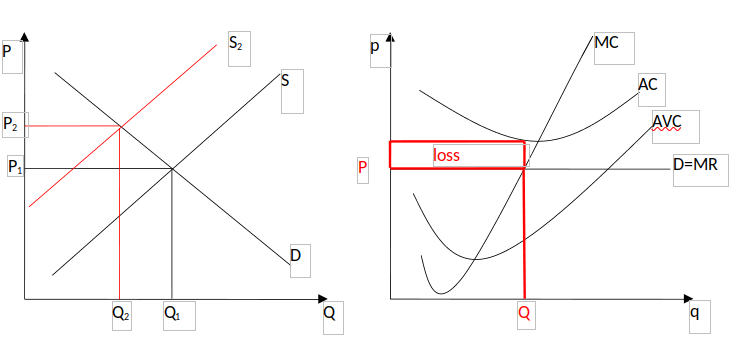
\includegraphics[width = \textwidth]{E2-2021Q1b.png}

\begin{parts}
\part On the diagram, show the profit or loss of the representative firm in its current short-run equilibrium position. Be sure to indicate whether it is a profit or a loss.
\part On the same diagram, show the output of the firm and the price that it would charge for this output.
\part If market demand does not change, and input prices do not change, in the long-run would you expect firms to enter or exit this market?   Briefly explain your answer.
\begin{solution} Firms will exit the market because they are making a loss. \end{solution}
\part Based on your response to question C., show on the demand and supply diagram what will happen in this market as it attains long-run equilibrium.
\begin{solution} As firms exit, supply shifts inward. This drives up the price and lowers the quantity. \end{solution}
\end{parts}

\question (2021Q3) You have a little sister at home who is taking AP Economics.  You get a text from her that reads, “What does the AVC curve have to do with whether a firm should shut down in the short-run, or keep producing output?”  Even though you and your little sister do not always get along, you decide to help her by explaining why the AVC curve shows a firm’s shut-down point.  What explanation do you text back?
\begin{solution} The shutdown point is defined by the point where price equals the \textbf{minimum} of the AVC. When the price falls below the shutdown point, the firm would be better off (or lose less money) by shutting down. When the price is above the shutdown point, the firm is better off (or loses less money) by producing some output even if it is making a loss.\end{solution}

\pagebreak
\question (2020Q7) You manage a firm that has developed a new drug that is quite successful at treating pancreatic cancer.  The firm has been awarded a patent.  The demand and cost curve for the firm you manage is shown below.

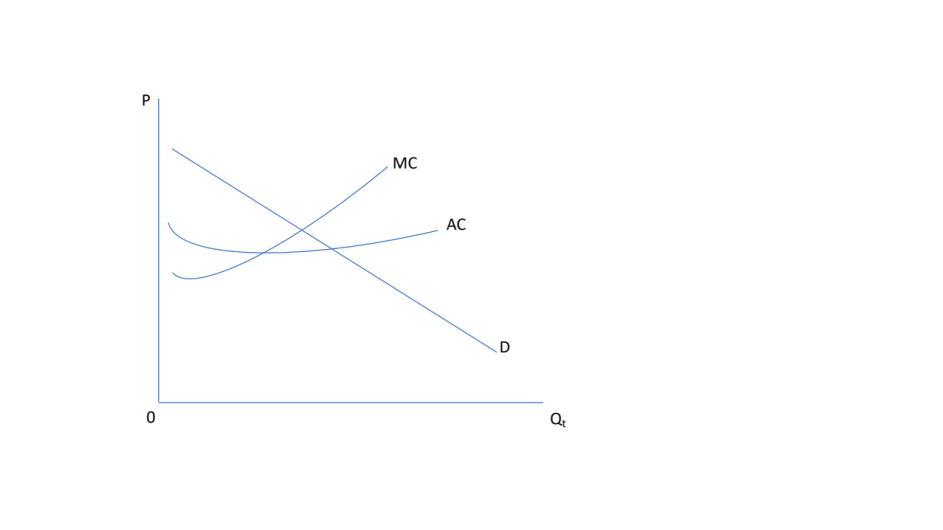
\includegraphics[width = \textwidth]{E2-2021Q7.png}

\begin{parts}
\part From the perspective of the firm that holds the patent, what is the economic consequence of the patent?
\begin{solution} The patent grants the firm monopoly power in producing the drug.\end{solution}
\part From the perspective of the economy in which the firm operates, what is the economic logic of having a patent system?
\begin{solution}Having a patent system gives entrepreneurs an incentive to innovate by granting them monopoly power -- and consequently economic profits -- for a fixed time period. \end{solution}
\part Based on the graph shown above, how would you describe the likely price the firm will charge for this breakthrough drug and what output will the firm produce?  What’s the basis for your answer? 
\begin{solution} The firm will produce where marginal cost is equal to marginal revenue. For a monopolist, the marginal revenue curve will lie inside the demand curve. The monopolist's price is \textbf{higher} and the quantity \textbf{lower} than in a competitive market. \end{solution}
\part After five years, a new drug is approved that is equally as effective at treating pancreatic cancer and does not violate your firm’s patent.  What do you expect will happen to the demand curve for your firm’s product as the new rival ramps up production of its product?
\begin{solution} The demand curve for your firms product will shift in (to the left) as the rival firm’s product is a substitute to your firm’s product. \end{solution}
\end{parts}

\end{questions}


\end{document}
